\begin{exercice}
La différence de $a-b$ est égale à 12. On augmente $a$ de 3 et on diminue $b$ de 4. Combien vaut la différence entre ces deux nouveaux nombres ?
\end{exercice}


\begin{exercice}[Triangle magique]
La somme des nombres de chaque côté du triangle est 2. Remplis les cases vides avec les nombres relatifs $(-2)$ ; $(-1)$ ; 1 ; 2 et 3.
\begin{center}
    \begin{tikzpicture}
    \node[name=b,priest,shirt=brown, hat=skin, cross=gray,mirrored,collar=brown, minimum size=1.5cm] at (2,0) {};
    \node[ellipse callout, draw,yshift= 1cm,xshift=-1cm, callout absolute pointer={(b.mouth)},    font=\footnotesize] {Ici, un triangle magique !};
    \end{tikzpicture}
\end{center}
\end{exercice}


\begin{exercice}[Le nombre $-21$...]
\begin{enumerate}
\item Écris le nombre $-21$ comme somme de deux nombres entiers relatifs consécutifs.
\item Écris le nombre $-21$ comme différence de deux carrés.
\end{enumerate}
\end{exercice}


\begin{exercice}
Complète les phrases suivantes :
\begin{enumerate}
\item $-21$ est la moitié de...
\item $-21$ est le triple de...
\item $-21$ est l'opposé de...
\end{enumerate}
\end{exercice}


\begin{exercice}[Choisir deux nombres]
\begin{enumerate}
\item Trouve deux nombres relatifs dont le produit est positif et la somme est négative.
\item Trouve deux nombres relatifs dont le produit est négatif et la somme est positive.
\item Trouve deux nombres relatifs dont le produit et la somme sont positifs.
\item Trouve deux nombres relatifs dont le produit et la somme sont négatifs.
\end{enumerate}
\end{exercice}



\begin{exercice}[Énigme]
Sachant que le produit de deux nombres $A$ et $B$ est positif et que leur somme est négative, quels sont les signes de $A$ et de $B$ ?
\end{exercice}



\begin{exercice}[Calculatrice]
Effectue à la calculatrice les calculs suivants :
\begin{enumerate}
\item $13 857 \times (-253)$
\item $\dfrac{-44980}{8996-10380}$
\item $312 -123 \times (-734)$
\item $\dfrac{-34 \times (-713)}{-68}$
\end{enumerate}
\end{exercice}



\begin{exercice}
Complète les carrés magiques suivants :
\begin{enumerate}
\item Pour l'addition :

\begin{center}
    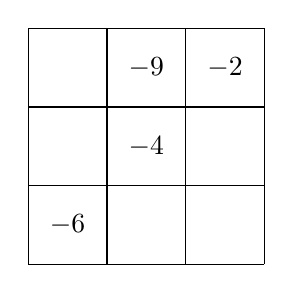
\begin{tikzpicture}
    \draw (0,0) grid (3,3);
    \draw (.5,.5) node {$-6$};
    \draw (1.5,1.5) node {$-4$};
    \draw (1.5,2.5) node {$-9$};
    \draw (2.5,2.5) node {$-2$};
    \end{tikzpicture}
\end{center}

\item Pour l'addition :

\begin{center}
    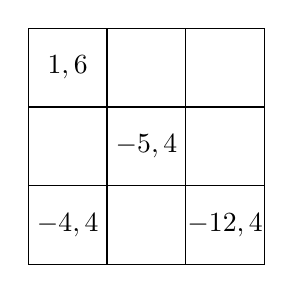
\begin{tikzpicture}
    \draw (0,0) grid (3,3);
    \draw (.5,.5) node {$-4,4$};
    \draw (2.5,.5) node {$-12,4$};
    \draw (1.5,1.5) node {$-5,4$};
    \draw (.5,2.5) node {$1,6$};
    \end{tikzpicture}
\end{center}

\end{enumerate}
\end{exercice}


\begin{exercice}[Signe]
$A$ est le produit de 24 nombres (non nuls) comportant 23 facteurs négatifs.
$B$ est le produit de 13 nombres (non nuls) comportant 11 facteurs négatifs. 
Donne, si c'est possible, le signe de :
\begin{colenumerate}{2}
\item $A \times B$
\item $A \div B$
\item $A -B$ 
\item $A^2$
\item $A + B$
\end{colenumerate}
\end{exercice}



\begin{exercice}[Coup de froid]
Chaque matin de la 1\up{ère} semaine du mois de février, Julie a relevé la température extérieure puis a construit le tableau suivant :

\vspace{.5em}
\renewcommand*\tabularxcolumn[1]{>{\centering\arraybackslash}m{#1}}
\renewcommand{\arraystretch}{1.6}
\begin{ctableau}{\linewidth}{8}
\hline
Jour & Lu & Ma & Me & Je & Ve & Sa & Di \\ \hline
T ($^\circ$C) & $-4$ & $-2$ & $-1$ & $+1$ & 0 & $+2$ & $-3$ \\ \hline
\end{ctableau}

Calcule la moyenne des températures relevées par Julie.
\end{exercice}




\begin{exercice}
Calcule les expressions suivantes en respectant les priorités :

$A = \dfrac{7-7\times 5}{6 \times 2 -5}$ 

$B = (4 -6) \times [5 + (3 -(-2)) \times 2]$

$C = \dfrac{-7 \times (-3) - (-3) \times (-5)}{(12 \div (-3) -2}$
\end{exercice}



\begin{exercice}
Effectue de deux manières différentes les calculs suivants :

$A = (-3) \times (5 -7)$

$B = 5 \times (-4 -3)$

$C = (-7 -2) \times (-3)$

$D = -3 \times ((-4) + (-2))$
\end{exercice}



\begin{exercice}
Calcul d'expressions.
\begin{enumerate}
\item Soit $D = (2\,x+3)^2 + (2\,x+3)(7\,x-2)$. 
Calculer $D$ pour $x = -4$.
\item Soit $E =36-(3\,x+5)^2$. 
Calculer $E$ pour $x = -2$.
\end{enumerate}
\end{exercice}



\begin{exercice}
En détaillant les étapes, calcule :
\begin{enumerate}
\item $A = 3x -7$ pour $x = + 2$ ;
\item $B = -2x -9$ pour $x = -5$ ;
\item $C = x^2 + 2$ pour $x = -1$.
\end{enumerate}
\end{exercice}




\begin{exercice}
Sachant que $a = 5$, $b = -3$ et $c = -10$, calcule les expressions suivantes :

$D = -2\,a$

$E = a -b$

$F = -3\,c + a$

$G = b -a -c$

$H = \dfrac{c}{a} + 2\,b$
\end{exercice}




\begin{exercice}
Calcule $b^2 -4 a\,c$ dans les cas suivants :
\begin{itemize}
    \item 1\up{er} cas : $a = 2$ ; $b = 3$ et $c = 5$.
    \item \up{e} cas : $a = -1$ ; $b = 2$ et $c = 3$.
    \item 3\up{e} cas : $a = 3$ ; $b = -2$ et $c = 2$.
\end{itemize}

\end{exercice}




\begin{exercice}[Conversion]
Aux États-Unis, la température $T$ est mesurée en degrés Fahrenheit. Voici la formule pour convertir une température $T_\text{°F}$ exprimée en degrés Fahrenheit (°F) en une température $T_\text{°C}$ équivalente exprimée en degrés Celsius (°C) :

\[  T_\text{°C} = \dfrac{(T_\text{°F}-32) \times 5}{9}\]

\begin{enumerate} \item À New-York est annoncée une température de 68°F. Convertis cette température en degrés Celsius à l'aide de la formule.
\item Même question pour une température de 23°F.
\item Voici la formule pour convertir une température exprimée en degrés Celsius (°C) en une température équivalente exprimée en degrés Fahrenheit (°F) :

\[ T_\text{°F} = T_\text{°C} \times 1,8 + 32 \]

Recopie puis complète le tableau suivant :

\vspace{.5em}
\renewcommand*\tabularxcolumn[1]{>{\centering\arraybackslash}m{#1}}
\renewcommand{\arraystretch}{1.6}
\begin{ctableau}{\linewidth}{6}
\hline
$T_\text{°C}$ & 0 & 5 & 10 & 15 & 20 \\ \hline
$T_\text{°F}$ & & & & & \\ \hline
\end{ctableau}

\item Place les données du tableau dans un repère similaire à celui ci-dessous.

\begin{center}
    \begin{tikzpicture}
    \draw [quadrillage] (0,0) grid (6,9);
    \axeX{0}{6}{0};
    \draw (2,0) node [below] {10};
    \draw (4,0) node [below] {20};
    \draw (6,0) node [right] {$T_\text{°C}$};
    \axeY{0}{9}{};
    \draw (0,2) node [left] {20};
    \draw (0,4) node [left] {40};
    \draw (0,6) node [left] {60};
    \draw (0,8) node [left] {80};
    \draw (0,9) node [above] {$T_\text{°F}$};
    \end{tikzpicture}
\end{center}

\item  À la vue du graphique, peut-on dire que les deux unités de température sont proportionnelles ? Justifie ta réponse.
\end{enumerate}
\end{exercice}

